\documentclass{beamer}

\usepackage{graphicx,hyperref,udesc,url}
\usepackage[utf8]{inputenc}
\usepackage[T1]{fontenc}
\usepackage{booktabs}
\usepackage[portuges]{babel}

\title[Subversion]{Sistema de Controle de Vers\~ao\\Apache Subversion}

\author[Rafael Castro, Lucas Mendes]{
    Rafael Castro, Lucas Mendes\\\medskip
    {\small \url{rafaelcgs10@gmail.com}} \\ 
{\small \url{lucasmpw@gmail.com}}}

\institute[UDESC]{
    Departamento de Ci\^encia da Computa\c{c}\~ao \\
    Centro de Ci\^encias e Tecnol\'ogias\\
Universidade do Estado de Santa Catarina}

\begin{document}

\begin{frame}
    \titlepage

\end{frame}

\begin{frame}
    \frametitle{Sum\'ario}
    \tableofcontents
\end{frame}

\section{Introdu\c{c}\~ao}


\begin{frame}
    \begin{figure}
        \centering
        
\includegraphics[width = 0.5\textwidth]{figures/Subversion}
    \end{figure}

    \frametitle{Hist\'oria}
    \begin{itemize}
        \item CollabNet fundou em 2000
        \item Foi aceito em uma incubadora do grupo Apache em 2009
    \end{itemize}
\end{frame}

\begin{frame}
    \frametitle{Motiva\c{c}\~ao}
    \begin{itemize}
        \item Competir com o CVS
        \item Proposta Livre
        \item Corrigir v\'arios problemas do CVS
        \item Novas funcionalidades
    \end{itemize}
\end{frame}

\begin{frame}
    \frametitle{Quem usa}
    \begin{itemize}
        \item Comunidade de Software Livre
        \item Grupo Apache
        \item Google
        \item Apple
    \end{itemize}
\end{frame}

\section{Caracter\'isticas em Particular}
\begin{frame}
    \frametitle{Pontos Importantes}
    \begin{itemize}
        \item Versionamento de diretórios
        \item Histórico de versões efetivo
        \item Manipulação consistente de dados
        \item Commit \'atomico
        \item Versionamento de metadados
        \item Ramificações e rotulagem eficiente
        \item Hackability
    \end{itemize}
\end{frame}


\begin{frame}
    \frametitle{Reposit\'orio}
    \begin{columns}

        \begin{column}{.555555\textwidth}
            \begin{block}{Arquitetura}
                \begin{columns}
                    \begin{column}{.5\textwidth}
                        \begin{itemize}
                            \item Cliente-Servidor
                        \end{itemize}
                    \end{column}
                    \begin{column}{.5\textwidth}
                        \begin{figure}
                            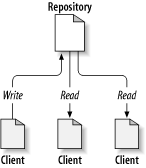
\includegraphics[width = 0.7\textwidth]{figures/repositorio}
                        \end{figure}
                    \end{column}
                \end{columns}
            \end{block}
        \end{column}

        \begin{column}{.5\textwidth}
            \begin{block}{Estrutura de arquivos}
                \begin{columns}
                    \begin{column}{.5\textwidth}
                        \begin{itemize}
                            \item \'Arvore de arquivos
                        \end{itemize}
                    \end{column}
                    \begin{column}{.5\textwidth}
                        \begin{figure}
                            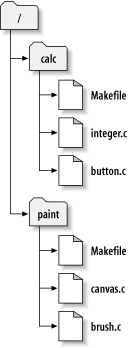
\includegraphics[width = 0.7\textwidth]{figures/arquivos}
                        \end{figure}
                    \end{column}
                \end{columns}
            \end{block}
        \end{column}
    \end{columns}
\end{frame}


\section{Conceitos B\'asicos}

\begin{frame}
    \frametitle{Reposit\'orio 2}

    \begin{columns}
        \begin{column}{.5\textwidth}
            \begin{itemize}
                \item Simples cole\c{c}\~ao de arquivos
                \item Centralizado
                \item Working copy - Os desenvolvedores trabalham com copias locais
            \end{itemize}
        \end{column}
        \begin{column}{.5\textwidth}
            \begin{block}{Pastas}
                \begin{enumerate}
                    \item .svn
                    \item trunk
                    \item branches
                    \item tags
                \end{enumerate}
            \end{block}
        \end{column}
    \end{columns}
\end{frame}

\begin{frame}
    \frametitle{Trunk e Branches}

    \begin{itemize}
        \item Linhas de desenvolvimento - Workflow padr\~ao
        \item Cheap and simple copy
    \end{itemize}
    \begin{columns}
        \begin{column}{.5\textwidth}
            \begin{figure}
                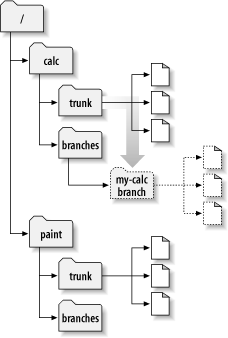
\includegraphics[width= 0.5\textwidth]{figures/copy}
            \end{figure}
        \end{column}
        \begin{column}{.5\textwidth}
        \begin{figure}
            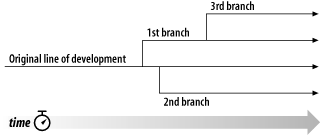
\includegraphics[width = 1.1\textwidth]{figures/branche}
        \end{figure}
    \end{column}
\end{columns}

\end{frame}

\begin{frame}
    \frametitle{Tags e Revis\~oes}
    \begin{columns}
        \begin{column}{.5\textwidth}
            \begin{block}{Tags}
                \begin{itemize}
                    \item Etiquetas de reiv\~oes
                \end{itemize}

            \end{block}
        \end{column}
    \end{columns}
\end{frame}

\section{Comandos B\'asicos}

\begin{frame}
    \frametitle{Checkout}

    This style file gives your slides some nice Radboud branding.
    When you know how to work with the Beamer package it is easy to use.
    Just add:\\ ~~~$\backslash$usepackage$\{$ru$\}$ \\ at the top of your file.
\end{frame}

\section{Conclus\~ao}

\begin{frame}
    \frametitle{Conclus\~ao}

    \begin{itemize}
        \item Easy to use
        \item Good results
    \end{itemize}
\end{frame}

\section{Refer\^encias}
\begin{frame}
    \frametitle{Refer\^encias}

    \begin{itemize}
        \item Easy to use
        \item Good results
    \end{itemize}
\end{frame}

\end{document}
